\documentclass[sigconf,nonacm]{acmart}
\settopmatter{printacmref=false, printccs=false, printfolios=true}
\renewcommand\footnotetextcopyrightpermission[1]{}
\pagestyle{plain}

\usepackage{booktabs}
\usepackage{multirow}
\usepackage{xspace}
\usepackage{tikz}
\usetikzlibrary{positioning,arrows.meta,fit,backgrounds,calc}
\graphicspath{{figures/}}
% generated by scripts/report_tables.py
\newcommand{\mrSiftPlannerMs}{0.31}
\newcommand{\mrSiftPlannerRec}{0.951}
\newcommand{\mrSiftThresholdMs}{5.55}
\newcommand{\mrSiftThresholdRec}{1.000}
\newcommand{\mrSiftFixedMs}{5.55}
\newcommand{\mrSiftFixedRec}{1.000}
\newcommand{\mrSiftGlobalMs}{6.39}
\newcommand{\mrSiftGlobalRec}{0.950}
\newcommand{\mrSiftOracleMs}{0.15}
\newcommand{\mrSiftOracleRec}{0.951}
\newcommand{\mrSiftSpeedup}{18.0}
\newcommand{\mrSiftOracleGap}{2.1}
\newcommand{\mrSiftGlobalSlowdown}{20.8}
\newcommand{\mrGistPlannerMs}{0.59}
\newcommand{\mrGistPlannerRec}{0.953}
\newcommand{\mrGistThresholdMs}{1.20}
\newcommand{\mrGistThresholdRec}{0.969}
\newcommand{\mrGistFixedMs}{2.26}
\newcommand{\mrGistFixedRec}{0.974}
\newcommand{\mrGistGlobalMs}{0.76}
\newcommand{\mrGistGlobalRec}{0.959}
\newcommand{\mrGistOracleMs}{0.33}
\newcommand{\mrGistOracleRec}{0.950}
\newcommand{\mrGistSpeedup}{2.0}
\newcommand{\mrGistOracleGap}{1.8}
\newcommand{\mrGistGlobalSlowdown}{1.3}
\newcommand{\mrGlovePlannerMs}{0.25}
\newcommand{\mrGlovePlannerRec}{0.954}
\newcommand{\mrGloveThresholdMs}{0.33}
\newcommand{\mrGloveThresholdRec}{0.962}
\newcommand{\mrGloveFixedMs}{3.55}
\newcommand{\mrGloveFixedRec}{1.000}
\newcommand{\mrGloveGlobalMs}{0.24}
\newcommand{\mrGloveGlobalRec}{0.950}
\newcommand{\mrGloveOracleMs}{0.13}
\newcommand{\mrGloveOracleRec}{0.950}
\newcommand{\mrGloveSpeedup}{1.3}
\newcommand{\mrGloveOracleGap}{2.0}
\newcommand{\mrGloveGlobalSlowdown}{1.0}
\newcommand{\mrDeepPlannerMs}{0.10}
\newcommand{\mrDeepPlannerRec}{0.949}
\newcommand{\mrDeepThresholdMs}{0.18}
\newcommand{\mrDeepThresholdRec}{0.966}
\newcommand{\mrDeepFixedMs}{3.23}
\newcommand{\mrDeepFixedRec}{1.000}
\newcommand{\mrDeepGlobalMs}{0.37}
\newcommand{\mrDeepGlobalRec}{0.938}
\newcommand{\mrDeepOracleMs}{0.06}
\newcommand{\mrDeepOracleRec}{0.950}
\newcommand{\mrDeepSpeedup}{1.7}
\newcommand{\mrDeepOracleGap}{1.6}
\newcommand{\mrDeepGlobalSlowdown}{3.6}
\newcommand{\mrYfccPlannerMs}{0.09}
\newcommand{\mrYfccPlannerRec}{0.965}
\newcommand{\mrYfccThresholdMs}{0.09}
\newcommand{\mrYfccThresholdRec}{0.959}
\newcommand{\mrYfccFixedMs}{1.73}
\newcommand{\mrYfccFixedRec}{1.000}
\newcommand{\mrYfccGlobalMs}{0.09}
\newcommand{\mrYfccGlobalRec}{0.966}
\newcommand{\mrYfccOracleMs}{0.06}
\newcommand{\mrYfccOracleRec}{0.951}
\newcommand{\mrYfccSpeedup}{1.1}
\newcommand{\mrYfccOracleGap}{1.4}
\newcommand{\mrYfccGlobalSlowdown}{1.1}
\newcommand{\mrSpeedupMin}{1.1}
\newcommand{\mrSpeedupMax}{18.0}
\newcommand{\mrOracleGapMin}{1.4}
\newcommand{\mrOracleGapMax}{2.1}
\newcommand{\mrWins}{32}
\newcommand{\mrCells}{35}
\newcommand{\liveSiftPlannerMs}{0.38}
\newcommand{\liveSiftPlannerRec}{0.957}
\newcommand{\liveSiftPlannerPninetyfive}{0.55}
\newcommand{\liveSiftPlannerIndependentRec}{0.999}
\newcommand{\liveSiftPlannerCorrelatedRec}{0.914}
\newcommand{\liveSiftThresholdMs}{5.36}
\newcommand{\liveSiftThresholdRec}{1.000}
\newcommand{\liveSiftThresholdPninetyfive}{14.57}
\newcommand{\liveSiftThresholdIndependentRec}{1.000}
\newcommand{\liveSiftThresholdCorrelatedRec}{1.000}
\newcommand{\liveSiftFixedMs}{5.29}
\newcommand{\liveSiftFixedRec}{1.000}
\newcommand{\liveSiftFixedPninetyfive}{14.51}
\newcommand{\liveSiftFixedIndependentRec}{1.000}
\newcommand{\liveSiftFixedCorrelatedRec}{1.000}
\newcommand{\liveSiftOverheadUs}{8}
\newcommand{\liveSiftSpeedup}{14.2}
\newcommand{\liveGistPlannerMs}{0.55}
\newcommand{\liveGistPlannerRec}{0.958}
\newcommand{\liveGistPlannerPninetyfive}{1.28}
\newcommand{\liveGistPlannerIndependentRec}{0.967}
\newcommand{\liveGistPlannerCorrelatedRec}{0.948}
\newcommand{\liveGistThresholdMs}{1.18}
\newcommand{\liveGistThresholdRec}{0.969}
\newcommand{\liveGistThresholdPninetyfive}{4.35}
\newcommand{\liveGistThresholdIndependentRec}{0.994}
\newcommand{\liveGistThresholdCorrelatedRec}{0.945}
\newcommand{\liveGistFixedMs}{2.11}
\newcommand{\liveGistFixedRec}{0.974}
\newcommand{\liveGistFixedPninetyfive}{7.59}
\newcommand{\liveGistFixedIndependentRec}{0.997}
\newcommand{\liveGistFixedCorrelatedRec}{0.950}
\newcommand{\liveGistOverheadUs}{25}
\newcommand{\liveGistSpeedup}{2.1}
\newcommand{\liveGlovePlannerMs}{0.26}
\newcommand{\liveGlovePlannerRec}{0.959}
\newcommand{\liveGlovePlannerPninetyfive}{0.57}
\newcommand{\liveGlovePlannerIndependentRec}{0.959}
\newcommand{\liveGlovePlannerCorrelatedRec}{0.959}
\newcommand{\liveGloveThresholdMs}{0.31}
\newcommand{\liveGloveThresholdRec}{0.962}
\newcommand{\liveGloveThresholdPninetyfive}{0.82}
\newcommand{\liveGloveThresholdIndependentRec}{0.970}
\newcommand{\liveGloveThresholdCorrelatedRec}{0.955}
\newcommand{\liveGloveFixedMs}{3.28}
\newcommand{\liveGloveFixedRec}{1.000}
\newcommand{\liveGloveFixedPninetyfive}{6.85}
\newcommand{\liveGloveFixedIndependentRec}{1.000}
\newcommand{\liveGloveFixedCorrelatedRec}{1.000}
\newcommand{\liveGloveOverheadUs}{8}
\newcommand{\liveGloveSpeedup}{1.2}
\newcommand{\liveDeepPlannerMs}{0.10}
\newcommand{\liveDeepPlannerRec}{0.953}
\newcommand{\liveDeepPlannerPninetyfive}{0.17}
\newcommand{\liveDeepPlannerIndependentRec}{0.980}
\newcommand{\liveDeepPlannerCorrelatedRec}{0.926}
\newcommand{\liveDeepThresholdMs}{0.18}
\newcommand{\liveDeepThresholdRec}{0.966}
\newcommand{\liveDeepThresholdPninetyfive}{0.47}
\newcommand{\liveDeepThresholdIndependentRec}{0.998}
\newcommand{\liveDeepThresholdCorrelatedRec}{0.934}
\newcommand{\liveDeepFixedMs}{3.25}
\newcommand{\liveDeepFixedRec}{1.000}
\newcommand{\liveDeepFixedPninetyfive}{6.89}
\newcommand{\liveDeepFixedIndependentRec}{1.000}
\newcommand{\liveDeepFixedCorrelatedRec}{1.000}
\newcommand{\liveDeepOverheadUs}{7}
\newcommand{\liveDeepSpeedup}{1.7}
\newcommand{\liveYfccPlannerMs}{0.09}
\newcommand{\liveYfccPlannerRec}{0.967}
\newcommand{\liveYfccPlannerPninetyfive}{0.20}
\newcommand{\liveYfccPlannerNativeRec}{0.967}
\newcommand{\liveYfccThresholdMs}{0.10}
\newcommand{\liveYfccThresholdRec}{0.959}
\newcommand{\liveYfccThresholdPninetyfive}{0.29}
\newcommand{\liveYfccThresholdNativeRec}{0.959}
\newcommand{\liveYfccFixedMs}{1.74}
\newcommand{\liveYfccFixedRec}{1.000}
\newcommand{\liveYfccFixedPninetyfive}{10.55}
\newcommand{\liveYfccFixedNativeRec}{1.000}
\newcommand{\liveYfccOverheadUs}{9}
\newcommand{\liveYfccSpeedup}{1.1}
\newcommand{\bestPreLow}{14}
\newcommand{\bestLowCells}{19}
\newcommand{\nDatasets}{5}

\renewcommand{\topfraction}{0.9}\renewcommand{\dbltopfraction}{0.9}
\renewcommand{\textfraction}{0.07}\renewcommand{\floatpagefraction}{0.85}\renewcommand{\dblfloatpagefraction}{0.85}
\setcounter{topnumber}{3}\setcounter{dbltopnumber}{3}\setcounter{totalnumber}{5}

\newcommand{\pre}{\textsc{Pre}\xspace}
\newcommand{\ivfpost}{\textsc{IVF-post}\xspace}
\newcommand{\ivfin}{\textsc{IVF-in}\xspace}
\newcommand{\pivfin}{\textsc{PIVF-in}\xspace}
\newcommand{\hnswpost}{\textsc{HNSW-post}\xspace}
\newcommand{\hnswin}{\textsc{HNSW-in}\xspace}
\newcommand{\repo}{\url{https://github.com/Ememusoh/vector-db-coen6317}}

\begin{document}

\title{Selectivity-Aware Filtered Vector Search:\\Choosing When to Filter Before, During, or After ANN Search}

\author{Emem Esther Usoh}
\affiliation{\institution{Concordia University}\city{Montr\'eal}\country{Canada}}
\author{Wassim Rahmoun}
\affiliation{\institution{Concordia University}\city{Montr\'eal}\country{Canada}}
\author{Ramprasad Giriraj}
\affiliation{\institution{Concordia University}\city{Montr\'eal}\country{Canada}}

\begin{abstract}
Filtered vector queries ask for the $k$ nearest neighbours of a query among the vectors that satisfy an attribute predicate. A system can filter \emph{before} the search (exact search over the matching vectors), \emph{after} it (approximate search, then discard non-matching results) or \emph{during} it (skip non-matching vectors inside the index). Which strategy is fastest depends on the filter's selectivity and, as we show, on where the matching vectors lie relative to the query. We implement six plans over IVF, an attribute-partitioned IVF and HNSW in a single measurement framework, and study them on \nDatasets{} dataset families with independent, correlated and native labels. No plan wins everywhere: the best plan's latency differs from exact pre-filtering by up to two orders of magnitude, in both directions. We then build a learned cost-model planner that predicts each plan's recall and latency from global and \emph{local} selectivity and selects plans with a Lagrangian rule calibrated to a recall target. At recall@10\,=\,0.95 it is \mrSpeedupMin--\mrSpeedupMax$\times$ faster than a tuned selectivity-threshold rule and within about 2$\times$ of a hindsight oracle. Local selectivity is what makes this work: without it the planner is up to \mrSiftGlobalSlowdown$\times$ slower.
\end{abstract}

\maketitle

% ---------------------------------------------------------------------------
\section{Problem and Motivation}

Vector databases increasingly serve \emph{hybrid} queries that combine similarity search with structured predicates, such as ``the 10 most similar images \textsf{WHERE} \textsf{country = 'Canada'}''. Approximate nearest-neighbour (ANN) indexes such as IVF~\cite{jegou2011pq} and HNSW~\cite{malkov2020hnsw} are built for unfiltered search, and a filter breaks their assumptions: IVF may probe clusters that contain no matching vectors, and an HNSW traversal may run out of matching neighbours before it reaches the query's region.

Production systems therefore combine three strategies~\cite{wei2020analyticdbv,wang2021milvus}. \emph{Pre-filtering} evaluates the predicate first and searches the matching vectors exactly, which is perfect in recall but costs time linear in the number of matches. \emph{Post-filtering} runs ANN search for more candidates than needed and discards those that fail the predicate, which is cheap for permissive filters but fails for selective ones. \emph{In-search filtering} checks the predicate inside the index traversal. The right choice changes with the query, so a query optimiser has to choose per query, as relational optimisers choose access paths~\cite{selinger1979access}. The usual heuristic switches on global selectivity alone: below a threshold, pre-filter; above it, use the index.

This project asks two questions. (1) \emph{When} is each strategy best, across indexes, selectivities, label distributions and datasets? (2) Can a cheap learned planner pick a plan per query that meets a recall target at lower latency than a tuned selectivity threshold? Our contributions:
\begin{itemize}
\item One framework that runs six filtered plans over IVF, attribute-partitioned IVF and HNSW, with shared Numba kernels that count every distance computation, so plans are compared on equal terms (\S\ref{sec:design}, \S\ref{sec:impl}).
\item A study on \nDatasets{} dataset families with synthetic labels that are independent of or correlated with the vectors, plus YFCC with native multi-label tags (\S\ref{sec:eval}).
\item A cost-model planner whose features include \emph{local selectivity}, i.e.\ how common the label is near the query. Its Lagrangian decision rule meets a recall target on average while spending latency only where it buys recall.
\end{itemize}

% ---------------------------------------------------------------------------
\section{Related Approaches}

\textbf{Strategy selection in systems.} AnalyticDB-V~\cite{wei2020analyticdbv} and Milvus~\cite{wang2021milvus} pick among pre-filtering, post-filtering and partition-based execution with cost models driven by predicate selectivity. Milvus also partitions data by a frequently filtered attribute. VBase~\cite{zhang2023vbase} instead integrates filtering into the index scan using relaxed monotonicity. These systems estimate selectivity globally. We show that, when labels correlate with the vectors, the \emph{local} density of matching vectors around the query matters as much.

\textbf{Filter-aware indexes.} Filtered-DiskANN~\cite{gollapudi2023filtereddiskann} builds graphs whose edges are aware of labels. NHQ~\cite{wang2023nhq} fuses attribute and vector distances in one graph. ACORN~\cite{patel2024acorn} densifies HNSW so that the subgraph induced by any predicate stays navigable. CAPS~\cite{gupta2023caps} partitions IVF lists by attribute, as our partitioned IVF does. SeRF~\cite{zuo2024serf} handles range predicates. These indexes improve one strategy. Our work is complementary: we treat them as plans and ask which to run for a given query. The NeurIPS'23 Big-ANN filtered track~\cite{simhadri2024neurips23} supplies our YFCC workload.

\textbf{Learned per-query decisions.} Learned adaptive early termination~\cite{li2020learned} predicts, per query, how much search an unfiltered ANN index needs. We predict per query \emph{which plan and budget} to use under a filter, using cheap features, and calibrate the decisions jointly to a recall target.

% ---------------------------------------------------------------------------
\section{System Design}\label{sec:design}

\begin{figure}[t]
\centering
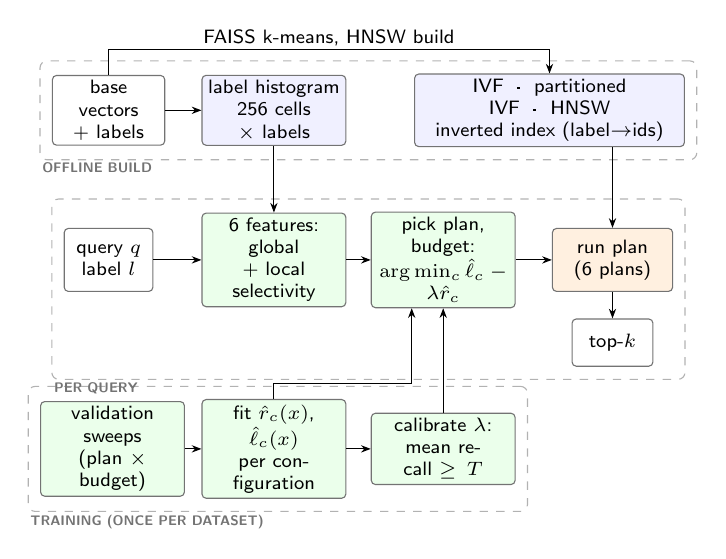
\begin{tikzpicture}[x=1mm, y=1mm, font=\sffamily\scriptsize, >={Stealth[length=3.5pt]},
  box/.style={draw=black!55, rounded corners=1.5pt, align=center, inner sep=1.8pt, minimum height=8mm, fill=white},
  idx/.style={box, fill=blue!6}, md/.style={box, fill=green!8}, pl/.style={box, fill=orange!12},
  lane/.style={draw=black!30, dashed, rounded corners=2.5pt, inner xsep=1.5mm, inner ysep=1.6mm},
  lbl/.style={font=\sffamily\tiny\bfseries, text=black!55, anchor=north west, inner sep=0.8pt}]
% offline build
\node[box, text width=13mm] (data) at (8,0) {base vectors\\+ labels};
\node[idx, text width=17mm] (hist) at (29,0) {label histogram\\256 cells $\times$ labels};
\node[idx, text width=33mm] (idx) at (64,0) {IVF \;·\; partitioned IVF \;·\; HNSW\\inverted index (label$\to$ids)};
\draw[->] (data) -- (hist);
\draw[->] (data.north) -- ++(0,3.2) -| node[pos=0.25, above, inner sep=1pt] {FAISS k-means, HNSW build} (idx.north);
% per query
\node[box, text width=10mm] (q) at (8,-19) {query $q$\\label $l$};
\node[md, text width=17mm] (feat) at (29,-19) {6 features: global\\+ local selectivity};
\node[md, text width=17mm] (dec) at (50.5,-19) {pick plan, budget:\\$\arg\min_c \hat\ell_c-\lambda\hat r_c$};
\node[pl, text width=14mm] (run) at (72,-19) {run plan\\(6 plans)};
\node[box, text width=9mm, minimum height=6mm] (out) at (72,-29.5) {top-$k$};
\draw[->] (q) -- (feat); \draw[->] (feat) -- (dec); \draw[->] (dec) -- (run); \draw[->] (run) -- (out);
\draw[->] (hist) -- (feat);
\draw[->] (idx.south -| run.north) -- (run.north);
% training
\node[md, text width=17mm] (sweep) at (8.5,-43) {validation sweeps\\(plan $\times$ budget)};
\node[md, text width=17mm] (models) at (29,-43) {fit $\hat r_c(x)$, $\hat\ell_c(x)$\\per configuration};
\node[md, text width=17mm] (lam) at (50.5,-43) {calibrate $\lambda$:\\mean recall $\ge T$};
\draw[->] (sweep) -- (models); \draw[->] (models) -- (lam);
\draw[->] (lam) -- (dec);
\draw[->] (models.north) -- ++(0,2) -| ([xshift=-4mm]dec.south);
\begin{scope}[on background layer]
\node[lane, fit=(data)(hist)(idx)] (L1) {};
\node[lane, fit=(q)(feat)(dec)(run)(out)] (L2) {};
\node[lane, fit=(sweep)(models)(lam)] (L3) {};
\end{scope}
\node[lbl] at (L1.south west) {OFFLINE BUILD};
\node[lbl] at (L2.south west) {PER QUERY};
\node[lbl] at (L3.south west) {TRAINING (ONCE PER DATASET)};
\end{tikzpicture}
\caption{System architecture. Offline, FAISS builds IVF and HNSW, from which we derive a label-partitioned IVF, an attribute inverted index and a coarse label histogram. Training sweeps every plan and budget on validation queries and fits the planner. Per query, the planner computes six features, picks a (plan, budget) and runs it.}
\label{fig:arch}
\end{figure}

\textbf{Problem.} Each base vector $x_i\in\mathbb{R}^d$ carries a label (synthetic datasets) or a set of tags (YFCC). A query $(q,l)$ asks for the $k=10$ nearest vectors under $L_2$ among $E_l=\{i: x_i \text{ has } l\}$, with selectivity $s_l=|E_l|/N$. A \emph{configuration} $c$ is a plan with a budget, and the planner must choose $c$ per query so that mean recall@10 over the workload reaches a target $T$ at minimum mean latency.

\subsection{Plans}
All six plans share the interface \texttt{search(q, label, k, budget)} (Fig.~\ref{fig:arch}).
\pre looks $E_l$ up in an inverted index and scans it exactly; its cost is $|E_l|\,d$ and its recall is 1.
\ivfpost and \hnswpost run unfiltered search for $k'=\lceil k/s_l\rceil$ candidates and keep the matching ones. If fewer than $k$ remain, they double $k'$ and the budget and search again, up to 12 rounds, as a client of a filter-unaware index would.
\ivfin probes \texttt{nprobe} lists but skips non-matching entries \emph{before} computing their distance, using a label array stored in list order.
\pivfin (attribute-partitioned IVF) sorts each list by label and keeps an offsets table of size nlist$\times(L{+}1)$, so a probe reads only the matching slice. This is the partition-by-attribute idea of~\cite{wang2021milvus,gupta2023caps}. It is defined only for single-valued labels.
\hnswin traverses the HNSW graph through all nodes but admits only matching nodes into the result heap, the common ``filter during traversal'' design. Its budget is \texttt{ef}.
Budgets range over powers of two: \texttt{nprobe}$\in\{1..1024\}$ and \texttt{ef}$\in\{10..1024\}$, giving 48 configurations per dataset (37 on YFCC, which has no \pivfin).

\subsection{Planner}
\textbf{Features.} For a query $(q,l)$ we compute six features, all as $\log_{10}$: the global selectivity $s_l$ and match count $|E_l|$; the \emph{local} selectivities $s^{(4)}_l$ and $s^{(16)}_l$, i.e.\ the fraction of vectors carrying $l$ in the 4 and 16 coarse k-means cells (out of 256) nearest to $q$; and the ratios $s^{(m)}_l/s_l$. Local selectivity is read from a precomputed $256\times L$ histogram, so the features cost 256 dot products. When labels correlate with the vectors, a label can be common overall yet absent near $q$. Index-based plans then lose recall or wander far, while \pre is unaffected. The ratio features expose exactly this case.

\textbf{Models.} For every configuration $c$ we fit two linear models on standardised features $z$, trained on the validation sweeps: expected recall $\hat r_c(x)=\sigma(w_c^\top z+b_c)$ by fractional logistic regression~\cite{papke1996fractional} on the measured recall values, and latency $\hat\ell_c(x)=\exp(v_c^\top z+a_c)$ by ridge regression on log-latency.

\textbf{Decision.} The planner picks
\begin{equation}
c^*(x)=\arg\min_{c}\; \hat\ell_c(x)-\lambda\,\hat r_c(x),
\end{equation}
which is the Lagrangian relaxation~\cite{everett1963lagrange} of ``minimise mean latency subject to mean recall $\ge T$''. Here $\lambda$ is the price of recall in milliseconds. It is set to the smallest value for which the choices made on 5-fold out-of-fold validation predictions reach mean recall $T$ (folds are grouped by query vector), found by bisection. The hindsight \emph{oracle} uses the same rule with measured instead of predicted values, so it lower-bounds the latency of any per-query policy. A first version of the planner instead picked the fastest configuration whose predicted probability of high recall exceeded a per-selectivity cutoff. Because every query then had to clear the bar on its own, it over-shot the target and was up to 3$\times$ slower (\S\ref{sec:eval}). The decision runs as a Numba loop over 37--48 configurations and, together with the features, takes \liveSiftOverheadUs\,$\mu$s per query.

\textbf{Baselines.} The \emph{threshold rule} pre-filters if $s_l<\theta$ and otherwise runs one fixed configuration. Both $\theta$ and that configuration are tuned on the same validation sweeps to meet $T$ at minimum latency, which is the selectivity-only heuristic described above, given every advantage of tuning. \emph{Best fixed} is the single fastest configuration that meets $T$. \emph{Global-only} is our planner restricted to the two global features.

% ---------------------------------------------------------------------------
\section{Implementation}\label{sec:impl}

\begin{figure}[t]
\centering
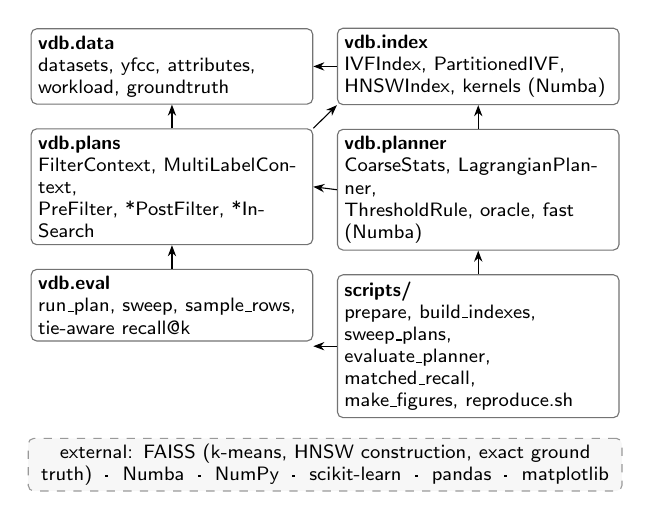
\begin{tikzpicture}[font=\sffamily\scriptsize, >={Stealth[length=4pt]},
  m/.style={draw=black!55, rounded corners=2pt, align=left, inner sep=2.5pt, text width=34mm, fill=white},
  ext/.style={draw=black!40, dashed, rounded corners=2pt, align=center, inner sep=2pt, fill=black!3}]
\node[m] (data) {\textbf{vdb.data}\\ datasets, yfcc, attributes,\\ workload, groundtruth};
\node[m, right=3mm of data] (index) {\textbf{vdb.index}\\ IVFIndex, PartitionedIVF,\\ HNSWIndex, kernels (Numba)};
\node[m, below=3mm of data] (plans) {\textbf{vdb.plans}\\ FilterContext, MultiLabelContext,\\ PreFilter, *PostFilter, *InSearch};
\node[m, below=3mm of index] (planner) {\textbf{vdb.planner}\\ CoarseStats, LagrangianPlanner,\\ ThresholdRule, oracle, fast (Numba)};
\node[m, below=3mm of plans] (eval) {\textbf{vdb.eval}\\ run\_plan, sweep, sample\_rows,\\ tie-aware recall@k};
\node[m, below=3mm of planner] (scripts) {\textbf{scripts/}\\ prepare, build\_indexes, sweep\_plans,\\ evaluate\_planner, matched\_recall,\\ make\_figures, reproduce.sh};
\node[ext, text width=74mm, anchor=north] (libs) at ($(eval.west |- scripts.south)!0.5!(scripts.south east)+(0,-2.5mm)$)
  {external: FAISS (k-means, HNSW construction, exact ground truth) \;·\; Numba \;·\; NumPy \;·\; scikit-learn \;·\; pandas \;·\; matplotlib};
\draw[->] (index.west) -- (data.east);
\draw[->] (plans) -- (data);
\draw[->] (plans.north east) -- (index.south west);
\draw[->] (planner.west) -- (plans.east);
\draw[->] (planner) -- (index);
\draw[->] (eval) -- (plans);
\draw[->] (scripts.west) -- (eval.east |- scripts.west);
\draw[->] (scripts) -- (planner);
\end{tikzpicture}
\caption{Implementation: Python packages (an arrow means ``uses'') and external libraries. Construction uses FAISS; every search, filter check and distance count runs in our own Numba kernels.}
\label{fig:impl}
\end{figure}

The system is about 3\,k lines of Python (Fig.~\ref{fig:impl}). FAISS~\cite{douze2024faiss} builds the IVF centroids and the HNSW graph (M\,=\,32, efConstruction\,=\,200). We extract its graph arrays and implement all search in Numba~\cite{lam2015numba} kernels (\texttt{vdb/index/kernels.py}): a bounded max-heap for results, a growable min-heap for HNSW candidates, an epoch-tagged visited array, and IVF list scans with an optional label check. Every kernel returns the number of distance computations it performed. Using our own kernels rather than FAISS's makes the six plans differ only in their algorithm, and lets the in-search plans check labels before computing distances. On unfiltered search our IVF and HNSW match FAISS's recall. IVF uses nlist\,$\approx4\sqrt{N}$ (4096 for 1M).

\texttt{FilterContext} bundles the vectors, labels, inverted index and indexes for one label scheme. \texttt{MultiLabelContext} handles YFCC's overlapping tags: before each query it writes the predicate into a per-vector label buffer, in both id order and IVF list order, which is the bitmap a filtered system would build. This step is untimed and identical for all plans. \texttt{CoarseStats} holds the 256-cell histogram and, with \texttt{LagrangianPlanner}, produces the per-query decision. Planners wrap the plans behind the same interface and record their decision overhead, so they are timed end-to-end.

\textbf{Workloads and ground truth.} The synthetic labels give four target labels exactly 50\%, 10\%, 1\% and 0.1\% of the vectors, and 39 filler labels take about 1\% each. \emph{Independent} labels are a random permutation. \emph{Correlated} labels are assigned to 1024 k-means cells ordered along the centroids' first principal component, so every label covers a compact region. Each of 1000 queries is paired with each target label, and queries are split 30/70 into validation and test \emph{by query vector}. For YFCC we take a uniform 1M subset of the 10M base and use the public queries that filter on a single tag. We group them into four selectivity bands (1--18\%, 0.1--1\%, 0.01--0.1\%, 0.001--0.01\%) of 500 queries each. Two-tag conjunctions are left out. Ground truth is the exact filtered top-100. Recall is \emph{tie-aware}: a returned vector counts if its distance is within the $k$-th true distance. Without this, exact search scores 0.998 on SIFT because of duplicate vectors.

\textbf{Reproducibility.} \texttt{scripts/reproduce.sh} runs every step for all datasets, skips steps whose outputs exist and records the software and hardware. The repository at \repo{} contains the code, README, tests (32 unit tests) and all results.

% ---------------------------------------------------------------------------
\section{Experimental Evaluation}\label{sec:eval}

\textbf{Setup.} All runs use one thread on an Apple M4 (16\,GB) with Python 3.12, Numba 0.68 and FAISS 1.16. Table~\ref{tab:datasets} lists the datasets: SIFT1M~\cite{jegou2011pq}, GIST (500K subset of 1M, $d=960$), GloVe-100~\cite{pennington2014glove} and Deep1M~\cite{babenko2016deep} from ANN-Benchmarks~\cite{aumuller2020annbench} (angular datasets normalised), and YFCC~\cite{thomee2016yfcc} as above. Validation sweeps use 200 queries per selectivity and test sweeps 100. Every method is trained on validation queries and evaluated on the disjoint test queries. We report recall@10, mean, median and p95 latency, distance computations, build time and memory.

\begin{table}[t]
\centering\scriptsize\setlength{\tabcolsep}{3pt}
\caption{Datasets and index construction (float32 vectors; IVF nlist\,=\,4096 for 1M; HNSW M\,=\,32, efC\,=\,200; FAISS builds use all 10 cores). The partitioned IVF adds only a 1.4\,MiB offsets table.}
\label{tab:datasets}
\begin{tabular}{lrrlrrrr}
\toprule
Dataset & $N$ & $d$ & Labels & Vec.\,MiB & IVF\,s & HNSW\,s & Graph\,MiB \\
\midrule
SIFT1M & 1M & 128 & synth. & 488 & 19 & 56 & 260 \\
GloVe-100 & 1M & 100 & synth. & 381 & 19 & 84 & 260 \\
Deep1M & 1M & 96 & synth. & 366 & 19 & 47 & 260 \\
\bottomrule
\end{tabular}

\end{table}

\begin{figure*}[t]
\centering
\includegraphics[width=\textwidth]{recall_latency_sift.pdf}
\caption{SIFT1M: recall@10 versus median latency for each plan as its budget grows, per selectivity (columns) and label scheme (rows). The square marker is exact pre-filtering. The dashed line is the 0.95 target.}
\label{fig:rl}
\end{figure*}

\subsection{No single plan wins}
Figure~\ref{fig:rl} shows the trade-off on SIFT, and Table~\ref{tab:best} gives the fastest plan reaching recall 0.95 for every dataset, label scheme and selectivity. At 50\% selectivity a graph or IVF plan is 6--96$\times$ faster than pre-filtering. At 0.1\%, pre-filtering scans only 1000 vectors and wins everywhere. In between, the partitioned IVF dominates at 10\% because it reads only matching entries. With correlated labels, the crossover moves: at 1\%, pre-filtering becomes the best plan on every synthetic dataset, because a query outside the label's region finds few matching vectors in the clusters or graph neighbourhood it explores. Index-based plans then show a \emph{bimodal} recall: near 1 for queries inside the region and near 0 outside, and post-filtering often hits its 12-round limit. Global selectivity cannot tell these two kinds of query apart.

\begin{table}[t]
\centering\scriptsize\setlength{\tabcolsep}{2.5pt}
\caption{Fastest plan (/budget) reaching recall@10\,$\ge$\,0.95 on test queries, and its median speed-up over pre-filtering when at least 1.5$\times$. YFCC columns are its four selectivity bands, from most to least common tag.}
\label{tab:best}
\begin{tabular}{llllll}
\toprule
Dataset & Labels & 50\% & 10\% & 1\% & 0.1\% \\
\midrule
SIFT1M & ind. & HNSW-in/32 (96$\times$) & PIVF-in/128 (55$\times$) & PIVF-in/256 (2$\times$) & Pre \\
SIFT1M & corr. & HNSW-in/64 (60$\times$) & PIVF-in/1024 (17$\times$) & Pre & Pre \\
GloVe-100 & ind. & IVF-post/256 (9$\times$) & PIVF-in/1024 (12$\times$) & Pre & Pre \\
GloVe-100 & corr. & HNSW-post/256 (6$\times$) & PIVF-in/1024 (10$\times$) & Pre & Pre \\
Deep1M & ind. & HNSW-in/32 (54$\times$) & PIVF-in/64 (72$\times$) & PIVF-in/256 & Pre \\
Deep1M & corr. & IVF-post/32 (21$\times$) & PIVF-in/1024 (16$\times$) & Pre & Pre \\
\bottomrule
\end{tabular}

\end{table}

\begin{figure*}[t]
\centering
\includegraphics[width=\textwidth]{matched_recall.pdf}
\caption{Matched recall. Each point is a method tuned on validation for one target in $\{0.85,\ldots,0.99\}$ and scored on the same test executions. Lower right is better.}
\label{fig:matched}
\end{figure*}

\begin{table*}[t]
\centering\small\setlength{\tabcolsep}{4pt}
\caption{Matched recall at target 0.95: mean recall@10 and mean latency (ms) on test queries, with every method scored on identical executions; planning overhead is included.}
\label{tab:matched}
\begin{tabular}{lrrrrrrrrrrr}
\toprule
 & \multicolumn{2}{c}{Planner} & \multicolumn{2}{c}{Threshold} & \multicolumn{2}{c}{Best fixed} & \multicolumn{2}{c}{Global-only} & \multicolumn{2}{c}{Oracle} & Speed-up \\
\cmidrule(lr){2-3} \cmidrule(lr){4-5} \cmidrule(lr){6-7} \cmidrule(lr){8-9} \cmidrule(lr){10-11}
Dataset & R@10 & ms & R@10 & ms & R@10 & ms & R@10 & ms & R@10 & ms & vs. thr. \\
\midrule
SIFT1M & 0.951 & 0.308 & 1.000 & 5.55 & 1.000 & 5.55 & 0.950 & 6.39 & 0.951 & 0.148 & 18.0$\times$ \\
GIST-500K & 0.953 & 0.587 & 0.969 & 1.20 & 0.974 & 2.26 & 0.959 & 0.762 & 0.950 & 0.333 & 2.0$\times$ \\
GloVe-100 & 0.954 & 0.250 & 0.962 & 0.327 & 1.000 & 3.55 & 0.950 & 0.238 & 0.950 & 0.126 & 1.3$\times$ \\
Deep1M & 0.949 & 0.104 & 0.966 & 0.181 & 1.000 & 3.23 & 0.938 & 0.369 & 0.950 & 0.064 & 1.7$\times$ \\
YFCC-1M & 0.965 & 0.086 & 0.959 & 0.093 & 1.000 & 1.73 & 0.966 & 0.093 & 0.951 & 0.060 & 1.1$\times$ \\
\bottomrule
\end{tabular}

\end{table*}

\subsection{Planner versus baselines}
\textbf{Matched recall.} To separate decision quality from timing noise, we score every method on the \emph{same} measured test executions: a method picks a configuration per query, and we look up that query's measured recall and latency (planning overhead added). Figure~\ref{fig:matched} sweeps the target, and Table~\ref{tab:matched} details $T=0.95$. The planner is faster than the tuned threshold rule in \mrWins{} of \mrCells{} (dataset, target) pairs. At $T=0.95$ the speed-up ranges from \mrSpeedupMin$\times$ to \mrSpeedupMax$\times$. The gain is largest on SIFT (\mrSiftPlannerMs{} vs.\ \mrSiftThresholdMs{} ms). There, no single fallback configuration meets the target on correlated 50\% queries, so the threshold rule degenerates to always pre-filtering, while the planner sends in-region queries to HNSW and out-of-region queries to \pre. The planner stays within \mrSiftOracleGap$\times$ (SIFT), \mrGloveOracleGap$\times$ (GloVe) and \mrDeepOracleGap$\times$ (Deep) of the hindsight oracle.

\textbf{Ablation: local selectivity.} The global-only planner is \mrSiftGlobalSlowdown$\times$ slower than the full planner on SIFT and \mrDeepGlobalSlowdown$\times$ slower on Deep, but no slower on GloVe (\mrGloveGlobalSlowdown$\times$). On SIFT and Deep, correlated queries at the same global selectivity need different plans, and only local selectivity separates them. On GloVe the best plans for in-region and out-of-region queries happen to coincide, so selectivity alone is enough.

\textbf{End-to-end.} Table~\ref{tab:live} runs the planner and the baselines live on the test queries. On SIFT the planner is \liveSiftSpeedup$\times$ faster than the threshold rule. On GloVe and Deep the live means are close (\liveGloveSpeedup$\times$ and \liveDeepSpeedup$\times$): the matched-recall gains of 1.3--1.7$\times$ are of the same order as run-to-run timing variation and the planner's \liveDeepOverheadUs\,$\mu$s overhead on sub-0.2\,ms queries. The Lagrangian rule meets the target \emph{on average}: it lets hard queries keep lower recall when raising it would be expensive. For example, SIFT correlated queries reach \liveSiftPlannerCorrelatedRec{} and independent ones \liveSiftPlannerIndependentRec. A per-selectivity $\lambda$ (an option of our implementation) guarantees the target for every group, at higher latency.

\begin{table}[t]
\centering\scriptsize\setlength{\tabcolsep}{2.6pt}
\caption{End-to-end live runs on test queries (target 0.95, calibration margin 0.005): recall@10 and mean/p95 latency (ms), planning time included; last column is the planner's planning time.}
\label{tab:live}
\begin{tabular}{lrrrrrrrr}
\toprule
 & \multicolumn{3}{c}{Planner} & \multicolumn{3}{c}{Threshold rule} & & \\
\cmidrule(lr){2-4} \cmidrule(lr){5-7}
Dataset & R@10 & mean & p95 & R@10 & mean & p95 & Speed-up & $\mu$s \\
\midrule
SIFT1M & 0.957 & 0.506 & 1.46 & 1.000 & 5.29 & 14.5 & 10.4$\times$ & 8 \\
GloVe-100 & 0.959 & 0.291 & 0.784 & 0.962 & 0.296 & 0.805 & 1.0$\times$ & 7 \\
Deep1M & 0.953 & 0.207 & 0.624 & 0.966 & 0.204 & 0.630 & 1.0$\times$ & 7 \\
\bottomrule
\end{tabular}

\end{table}

% ---------------------------------------------------------------------------
\section{Analysis and Lessons Learned}

\textbf{Why the planner wins, and where it does not.} The planner's advantage comes from queries whose best plan differs at the \emph{same} global selectivity. Correlated labels create such queries in large numbers. Independent labels create almost none: there the threshold rule is already near-optimal, and the planner merely matches it. YFCC's real tags behave in between: tags are correlated with image content, but a tag's matches are spread over many regions. The remaining gap to the oracle (about 2$\times$) comes from latency the linear models cannot predict, notably HNSW's long tail on queries just outside a label's region, where in-search traversal explores many non-matching nodes.

\textbf{Limitations.} The planner needs a sweep of every configuration on validation queries, about an hour per dataset. It must be retrained when labels or indexes change. YFCC's two-tag conjunctions, range predicates and multi-threaded execution are out of scope. Synthetic labels control selectivity exactly but only approximate real attribute distributions.

\textbf{Lessons learned.}
(1) \emph{Selectivity is a property of the query, not only of the label.} The local-selectivity features, which cost a few microseconds, account for up to \mrSiftGlobalSlowdown$\times$ of the planner's gain. A global-selectivity estimate, as used by current optimisers, misses the correlated case entirely.
(2) \emph{Calibrate the aggregate, not each decision.} Requiring each query to clear a recall bar on its own made our first planner over-shoot the target, at 0.967 instead of 0.95 on SIFT, and up to 3$\times$ slower. Pricing recall with one multiplier, the rule the oracle uses, closed most of the gap.
(3) \emph{Fair comparison needs shared kernels and careful recall.} Mixing FAISS's optimised search with hand-written filtered search would have measured implementation quality rather than plans. Counting distances in one set of kernels exposed, for example, that post-filtering's cost is dominated by re-searches. Tie-aware recall was needed for exact search to score 1.0.
(4) \emph{Partitioning by attribute is cheap but narrow.} The partitioned IVF costs only a 1.4\,MiB offsets table and wins at moderate selectivity. However, it requires one value per vector and does not apply to YFCC's overlapping tags.

% ---------------------------------------------------------------------------
\section{Contributions and Availability}

Code, data preparation, results and figures are available at \repo. \texttt{scripts/reproduce.sh} regenerates every table and figure in this report. Table~\ref{tab:contrib} lists the contributions of each member.

\begin{table}[t]
\centering\small
\caption{Team contributions.}
\label{tab:contrib}
\begin{tabular}{p{0.26\columnwidth}p{0.64\columnwidth}}
\toprule
Member & Contributions \\
\midrule
Emem E.\ Usoh & System design; data layer, indexes and Numba kernels, filtered plans, planner and baselines; experiments; figures; report \\
Wassim Rahmoun & \textit{[to be completed]} \\
Ramprasad Giriraj & \textit{[to be completed]} \\
\bottomrule
\end{tabular}
\end{table}

\bibliographystyle{ACM-Reference-Format}
\bibliography{refs}

\end{document}
